\documentclass[12pt]{article}

\usepackage[utf8]{inputenc}
\usepackage{amsmath, amssymb, amsfonts, cancel}
\usepackage{graphicx}
\usepackage[letterpaper, left=1in, right=1in, top=1in, bottom=1in]{geometry}
\usepackage{booktabs}
\usepackage{multirow}
\usepackage{float}
\usepackage{caption}
\usepackage{colortbl}
\usepackage{xcolor}
\definecolor{paleYellow}{RGB}{255,255,180}
\usepackage{physics}
\usepackage{hyperref}
\usepackage[spanish]{babel}

\title{
Práctica 4: ACL estándar\\[0.5em]
\large Interacción de redes
}

\author{
Jorge Alberto Suarez Saldana\\
\small Matrícula: 355992\\
\small Profesor: Raymundo Antonio González Grimaldo
}

\date{\today}

\begin{document}
\maketitle

\section{Topología de la red}

La topología utilizada para la práctica está compuesta por tres routers, cuatro
switches y seis dispositivos finales. RouterB funciona como router intermedio
entre RouterA y RouterC, mientras que RouterA y RouterC proporcionan
conectividad a las redes LAN.

\begin{figure}[H]
    \centering
    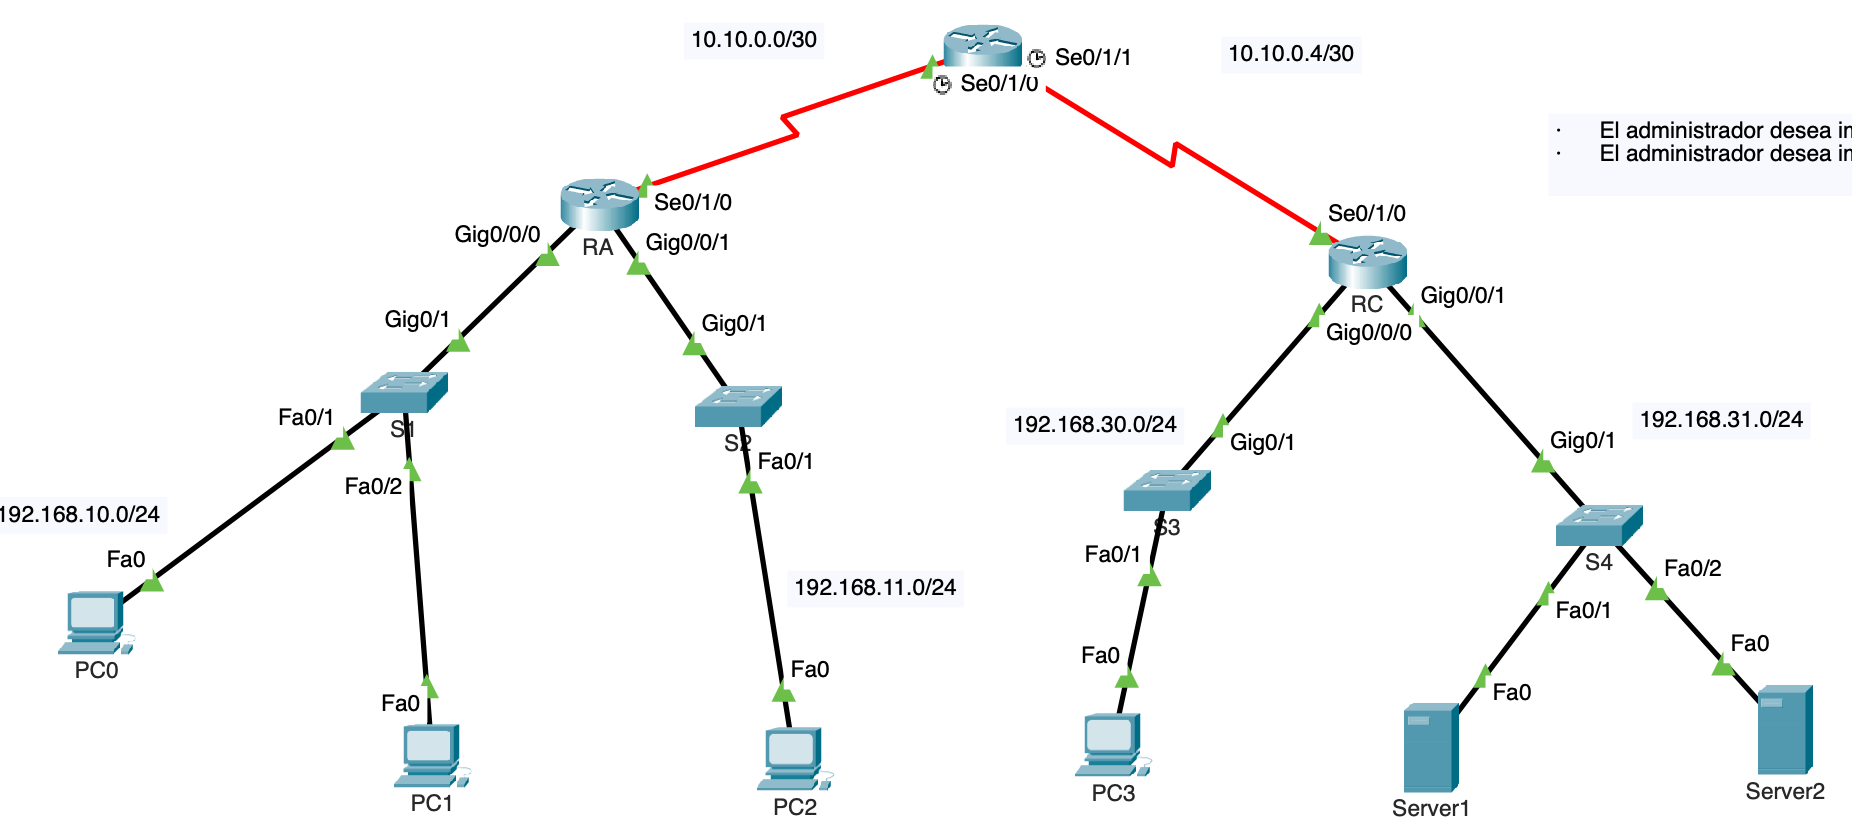
\includegraphics[width=\textwidth]{topologia.png}
    \caption{Topología de red utilizada en la práctica.}
    \label{fig:topologia}
\end{figure}

Las conexiones entre los dispositivos y las redes utilizadas se muestran en la
Tabla~\ref{tab:direccionamiento}.

\begin{table}[H]
    \centering
    \caption{Direccionamiento de la topología.}
    \label{tab:direccionamiento}
    \small
    \begin{tabular}{llll}
        \toprule
        \textbf{Dispositivo} & \textbf{Interfaz} & \textbf{Dirección IP} & \textbf{Red} \\
        \midrule
        RouterA & Se0/1/0 & -- & 10.10.0.0/30 \\
        RouterB & Se0/1/0 & -- & 10.10.0.0/30 \\
        RouterB & Se0/1/1 & -- & 10.10.0.4/30 \\
        RouterC & Se0/1/0 & -- & 10.10.0.4/30 \\
        RouterA & Gi0/0/0 & -- & 192.168.10.0/24 \\
        RouterA & Gi0/0/1 & -- & 192.168.11.0/24 \\
        RouterC & Gi0/0/0 & -- & 192.168.30.0/24 \\
        RouterC & Gi0/0/1 & -- & 192.168.31.0/24 \\
        \midrule
        PC0 & NIC & 192.168.10.100 & 192.168.10.0/24 \\
        PC1 & NIC & 192.168.10.101 & 192.168.10.0/24 \\
        PC2 & NIC & 192.168.11.100 & 192.168.11.0/24 \\
        PC3 & NIC & 192.168.30.100 & 192.168.30.0/24 \\
        Server1 & NIC & 192.168.31.2 & 192.168.31.0/24 \\
        Server2 & NIC & 192.168.31.32 & 192.168.31.0/24 \\
        \bottomrule
    \end{tabular}
\end{table}

\section{Objetivo}

El objetivo de la práctica es implementar y verificar listas de control de
acceso (ACL) estándar en los routers de la topología.

Las restricciones solicitadas por el administrador son las siguientes:

\begin{enumerate}
    \item Impedir que el tráfico originado en la red
    \texttt{192.168.10.0/24} llegue a la red
    \texttt{192.168.30.0/24}, con la excepción del host
    \texttt{192.168.10.101}, que debe conservar el acceso.

    \item Impedir que el tráfico originado en las direcciones
    \texttt{192.168.31.2} a \texttt{192.168.31.31} llegue a la red
    \texttt{192.168.11.0/24}.
\end{enumerate}

Una ACL estándar solamente permite tomar decisiones basándose en la dirección
IP de origen. Por esta razón, la ubicación de la ACL dentro de la topología es
fundamental para conseguir que las restricciones afecten únicamente a los
destinos solicitados.

\section{Pruebas previas a la configuración}

Antes de configurar las ACL se realizaron pruebas de conectividad entre los
hosts involucrados. El propósito de estas pruebas fue comprobar que existía
conectividad entre las redes antes de aplicar las restricciones.

La Figura~\ref{fig:previo} muestra los resultados de las pruebas de
conectividad realizadas antes de implementar las ACL.

\begin{figure}[H]
    \centering
    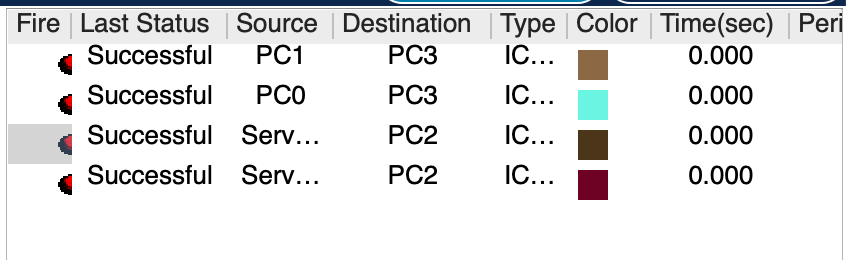
\includegraphics[width=\textwidth]{previoConfig.png}
    \caption{Pruebas de conectividad previas a la configuración de las ACL.}
    \label{fig:previo}
\end{figure}

Estas pruebas establecen una referencia para comparar el comportamiento de la
red antes y después de aplicar las listas de control de acceso.

\section{Configuración de las ACL}

\subsection{ACL en RouterC}

La primera restricción establece que los dispositivos de
\texttt{192.168.10.0/24} no deben poder comunicarse con la red
\texttt{192.168.30.0/24}, excepto el host
\texttt{192.168.10.101}.

Debido a que se utiliza una ACL estándar, la lista solamente puede evaluar la
dirección de origen. Por ello, la ACL se colocó en RouterC, en la interfaz
\texttt{Gi0/0/0}, que es la interfaz conectada directamente a la red
\texttt{192.168.30.0/24}. La ACL se aplica en dirección de salida.

La configuración utilizada fue:

\begin{verbatim}
RouterC(config)# access-list 1 permit host 192.168.10.101
RouterC(config)# access-list 1 deny 192.168.10.0 0.0.0.255
RouterC(config)# access-list 1 permit any

RouterC(config)# interface GigabitEthernet0/0/0
RouterC(config-if)# ip access-group 1 out
\end{verbatim}

El orden de las entradas es importante. Primero se permite explícitamente el
host \texttt{192.168.10.101}. Posteriormente se deniega el resto de la red
\texttt{192.168.10.0/24}.

Finalmente se utiliza \texttt{permit any} para permitir el tráfico proveniente
de otras redes. Esto es necesario debido al funcionamiento de las ACL, que
poseen implícitamente un \texttt{deny any} al final de la lista.

\subsection{ACL en RouterA}

La segunda restricción establece que los hosts con direcciones comprendidas
entre \texttt{192.168.31.2} y \texttt{192.168.31.31} no deben poder alcanzar
la red \texttt{192.168.11.0/24}.

La ACL se colocó en RouterA, sobre la interfaz \texttt{Gi0/0/1}, conectada a
la red \texttt{192.168.11.0/24}, y se aplicó en dirección de salida.

El rango solicitado no puede representarse mediante una única entrada de ACL
estándar sin incluir direcciones adicionales. Por ello, el rango se dividió
utilizando varias wildcard masks:

\begin{table}[H]
    \centering
    \caption{Descomposición del rango de direcciones bloqueadas.}
    \label{tab:rango}
    \small
    \begin{tabular}{lll}
        \toprule
        \textbf{Rango} & \textbf{Dirección base} & \textbf{Wildcard mask} \\
        \midrule
        2--3 & 192.168.31.2 & 0.0.0.1 \\
        4--7 & 192.168.31.4 & 0.0.0.3 \\
        8--15 & 192.168.31.8 & 0.0.0.7 \\
        16--31 & 192.168.31.16 & 0.0.0.15 \\
        \bottomrule
    \end{tabular}
\end{table}

La configuración utilizada fue:

\begin{verbatim}
RouterA(config)# access-list 2 deny 192.168.31.2 0.0.0.1
RouterA(config)# access-list 2 deny 192.168.31.4 0.0.0.3
RouterA(config)# access-list 2 deny 192.168.31.8 0.0.0.7
RouterA(config)# access-list 2 deny 192.168.31.16 0.0.0.15
RouterA(config)# access-list 2 permit any

RouterA(config)# interface GigabitEthernet0/0/1
RouterA(config-if)# ip access-group 2 out
\end{verbatim}

De esta manera, las direcciones \texttt{192.168.31.2} a
\texttt{192.168.31.31} son bloqueadas, mientras que las direcciones fuera
del rango pueden continuar comunicándose con la red
\texttt{192.168.11.0/24}.

\section{Pruebas posteriores a la configuración}

Después de aplicar las ACL se realizaron nuevamente pruebas de conectividad.
Los resultados permitieron comprobar tanto los casos que debían ser
bloqueados como las excepciones que debían permanecer permitidas.

\begin{table}[H]
    \centering
    \caption{Pruebas de conectividad posteriores a la configuración.}
    \label{tab:pruebas}
    \small
    \begin{tabular}{llll}
        \toprule
        \textbf{Origen} & \textbf{Destino} & \textbf{Resultado esperado}
        & \textbf{Resultado} \\
        \midrule
        PC1
        & PC3
        & Permitido
        & Correcto \\
        
        PC0
        & PC3
        & Bloqueado
        & Correcto \\
        
        Server1
        & PC2
        & Bloqueado
        & Correcto \\
        
        Server2
        & PC2
        & Permitido
        & Correcto \\
        \bottomrule
    \end{tabular}
\end{table}

Las direcciones utilizadas en las pruebas fueron:

\begin{itemize}
    \item PC1: \texttt{192.168.10.101}
    \item PC0: \texttt{192.168.10.100}
    \item PC3: \texttt{192.168.30.100}
    \item Server1: \texttt{192.168.31.2}
    \item Server2: \texttt{192.168.31.32}
    \item PC2: \texttt{192.168.11.100}
\end{itemize}

La Figura~\ref{fig:resultados} presenta las pruebas realizadas después de
aplicar las listas de control de acceso.

\begin{figure}[H]
    \centering
    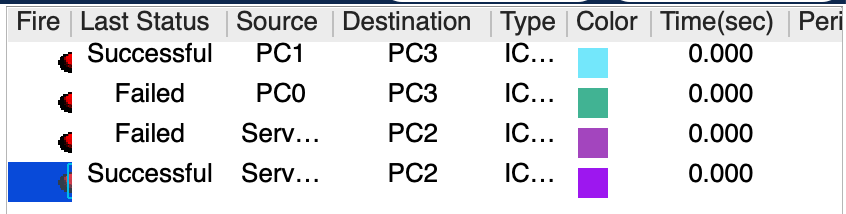
\includegraphics[width=\textwidth]{resultados.png}
    \caption{Resultados de las pruebas de conectividad después de configurar las ACL.}
    \label{fig:resultados}
\end{figure}

Los resultados coinciden con el comportamiento esperado. En particular,
PC1, cuya dirección es \texttt{192.168.10.101}, conserva la comunicación con
PC3 debido a que fue configurado como una excepción. PC0, cuya dirección es
\texttt{192.168.10.100}, queda bloqueado al intentar comunicarse con PC3.

De manera similar, Server1, con dirección \texttt{192.168.31.2}, queda
bloqueado al intentar comunicarse con PC2, mientras que Server2, con dirección
\texttt{192.168.31.32}, conserva la conectividad debido a que su dirección
está fuera del rango restringido.

\section{Verificación mediante \texttt{show access-lists}}

Además de las pruebas mediante \texttt{ping}, se verificó que los paquetes
fueran procesados por las ACL utilizando el comando
\texttt{show access-lists}.

\subsection{RouterA}

En RouterA se ejecutó:

\begin{verbatim}
RouterA# show access-lists 2
\end{verbatim}

La salida obtenida se muestra en la Figura~\ref{fig:aclA}.

\begin{figure}[H]
    \centering
    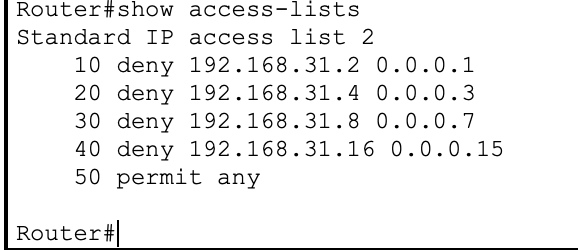
\includegraphics[width=\textwidth]{listaAccesosRouterA.png}
    \caption{Salida de \texttt{show access-lists} en RouterA.}
    \label{fig:aclA}
\end{figure}

Los contadores asociados a las entradas de la ACL permiten comprobar que las
reglas fueron utilizadas durante las pruebas de conectividad. En particular,
los intentos realizados desde las direcciones comprendidas dentro del rango
bloqueado incrementaron los contadores correspondientes a las entradas
\texttt{deny}.

\subsection{RouterC}

En RouterC se ejecutó:

\begin{verbatim}
RouterC# show access-lists 1
\end{verbatim}

La salida obtenida se muestra en la Figura~\ref{fig:aclC}.

\begin{figure}[H]
    \centering
    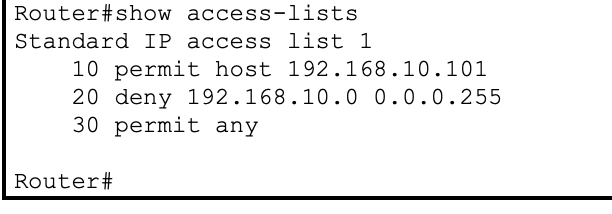
\includegraphics[width=\textwidth]{listaAccesosRouterC.png}
    \caption{Salida de \texttt{show access-lists} en RouterC.}
    \label{fig:aclC}
\end{figure}

En este caso, los contadores permiten verificar el procesamiento tanto de la
excepción \texttt{192.168.10.101} como del tráfico proveniente del resto de
la red \texttt{192.168.10.0/24}.

\section{Análisis}

Las pruebas realizadas permitieron comprobar el funcionamiento de las ACL
estándar y la importancia de seleccionar correctamente la interfaz y la
dirección de aplicación de una ACL.

En RouterC, la ACL fue colocada en la interfaz que conduce hacia
\texttt{192.168.30.0/24}. Esto permitió bloquear el tráfico proveniente de
\texttt{192.168.10.0/24} únicamente cuando dicho tráfico tenía como destino
esa red.

La excepción se implementó colocando la entrada:

\begin{verbatim}
permit host 192.168.10.101
\end{verbatim}

antes de la entrada que bloquea toda la red
\texttt{192.168.10.0/24}. Esto es necesario porque las ACL se procesan de
arriba hacia abajo y el router utiliza la primera entrada que coincide con el
paquete.

En RouterA, el rango de direcciones \texttt{192.168.31.2} a
\texttt{192.168.31.31} tuvo que dividirse en cuatro bloques debido a las
características de las wildcard masks. El host Server2,
\texttt{192.168.31.32}, quedó fuera de estos bloques y, por lo tanto, no fue
afectado por las reglas \texttt{deny}.

Finalmente, la entrada \texttt{permit any} utilizada en ambas ACL permite que
el tráfico que no coincide con las reglas de bloqueo continúe siendo
procesado. Sin esta entrada, el \texttt{deny any} implícito al final de la
ACL impediría el tráfico restante.

\section{Conclusiones}

La práctica permitió implementar dos ACL estándar para controlar el acceso
entre diferentes redes de la topología.

La primera ACL restringió el acceso desde
\texttt{192.168.10.0/24} hacia \texttt{192.168.30.0/24}, manteniendo como
excepción al host \texttt{192.168.10.101}. La segunda ACL restringió el acceso
desde las direcciones \texttt{192.168.31.2} a
\texttt{192.168.31.31} hacia \texttt{192.168.11.0/24}, manteniendo fuera de
la restricción al host \texttt{192.168.31.32}.

Los resultados de las pruebas mediante \texttt{ping} coincidieron con las
reglas establecidas y las salidas de \texttt{show access-lists} permitieron
verificar que las entradas de las ACL fueron utilizadas durante las pruebas.

De esta manera, se comprobó experimentalmente el funcionamiento de las ACL
estándar, el procesamiento secuencial de sus entradas, el uso de wildcard
masks para representar rangos de direcciones y la importancia de colocar la
ACL en la interfaz y dirección adecuadas.

\end{document}